In the previous sections, we implicitly assumed that the raw movie of fluorescence measurements collected by the experimenter had undergone two stages of pre-processing.  First, the movie was segmented, to determine regions-of-interest (ROIs).  This yields a vector, $\vF_t$, corresponding to the fluorescence intensity at time $t$ for each of the $N_p$ pixels in the ROI.  Second, we projected that vector into a scalar, yielding $F_t$, the assumed input.  In this section, we still assume that somebody has gone through our movies and performed some segmentation, but we do not assume that they have projected the vector $\vF_t$ into a scalar $F_t^{proj}$.  Formally, we posit a more general model:

\begin{align} \label{eq:bF}
\vF_t &= \valpha (C_t + \beta) +  \sig \vec{\varepsilon}_t, \qquad &\vec{\varepsilon}_t \sim \mathcal{N}(\vec{0},\bI)   
\end{align}

\noindent where $\vF_t$, $\valpha$, $\vec{\varepsilon}_t$, and $\vec{0}$  are all column vectors of length $N_p$, and $\bI$ is an $N_p \times N_p$ identity matrix.  This model follows because the fluorescence at any individual pixel may be composed of a static element, $\beta$, and a dynamic element, that we assume is purely due to calcium fluctuations, $C_t$.  Further, we have assumed that the noise is uncorrelated and has the same variance, $\sig^2$, in each pixel (an assumption that can be relaxed quite easily).  Performing inference in this more general model proceeds nearly identical as before:

\begin{align} 
\hbC_{\zzz} 
&= \az  \frac{1}{2 \sig^2} \norm{\vec{\bF} - \valpha (\bC\T +\beta\ve{1}\T)}^2 + (\bM \bC )\T \blam  - \zzz \log(\bM \bC)\T\ve{1},  \label{eq:eta4}\\
\ve{g} &= -\frac{\balpha}{\sig^2}(\bF -\balpha({\hbC\T}_{\zzz} + \beta)) + \ve{M}\T\blam - \zzz \ve{M}\T (\ve{M} \hbC_{\zzz})^{-1} \label{eq:g2} \\
\ve{H} &= \frac{\balpha\T \balpha}{\sig^2} \ve{I} + \zzz \ve{M}\T (\ve{M} \hbC_{\zzz})^{-2} \ve{M} \label{eq:H2}
\end{align}

Figure \ref{fig:spatial} demonstrates the utility of this generalization.  The top row shows different depictions of an ROI containing a single neuron.  On the far left panel is the ``true'' spatial filter.  We modeled the true spatial filter as a sum of Gaussians: a positively weighted small variance Gaussian, and a negatively weighted large variance Gaussian.  We chose this model based on our empirical observations that often pixels immediately around a neuron exhibit calcium sensitive fluctuations that are anti-correlated with the pixels on the neuron, probably due to the calcium influx from the vicinity of the neuron. The mean frame (second panel from left) looks very similar to the true spatial filter, as individual frames are effectively just modulating the magnitude of the spatial filter, and adding noise.  Typically, to obtain an ROI, one would simply identify the pixels with high positive values from the mean frame, and average them together (third panel from left).  Such an approach yields the 1-dimensional fluorescence projection depicted on the left, the typical projection, $F_t^{typ}$, with its associated inferred spike train beneath.  Using the true spatial filter to project $\vec{\bF}$ onto a 1-dimensional fluorescence time series results on the right, the optimal projection, $F_t^{opt}$, with its associated inferred spike train beneath.  It should be clear that using the true spatial filter improves the SNR of the fluorescence signal, and therefore, the inferred spike train accuracy.

\begin{figure}[H]
\centering 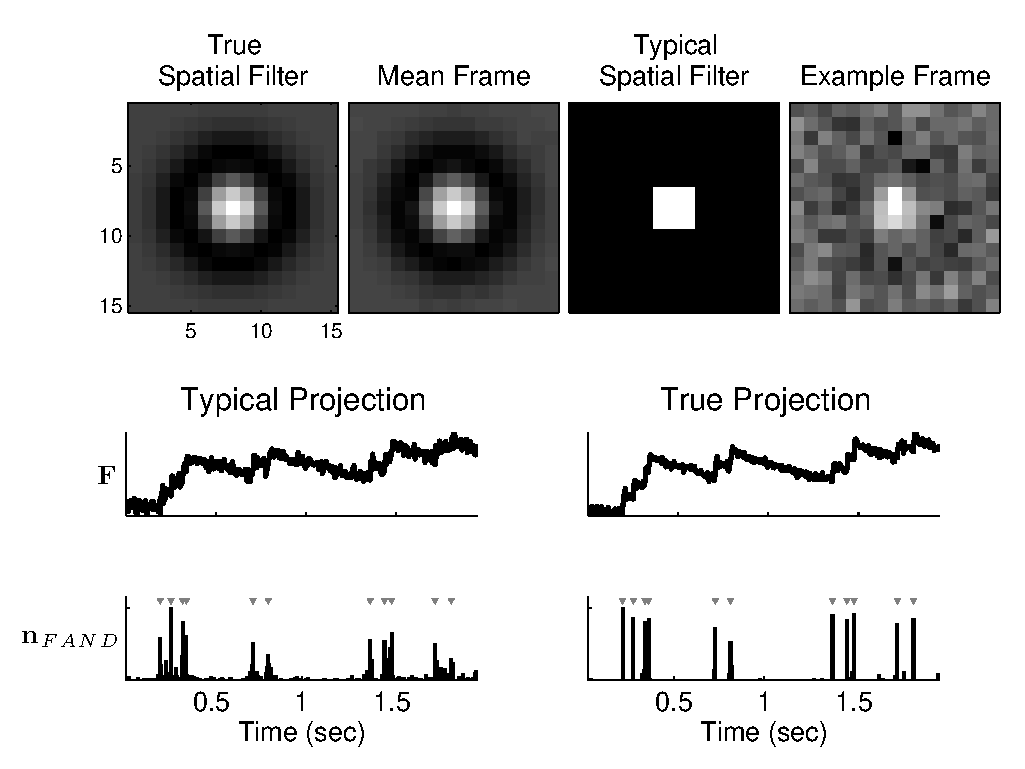
\includegraphics[width=.9\linewidth]{../figs/spatial}
\caption{A simulation demonstrating that using a better spatial filter can significantly enhance the effective SNR (see Supplementary Movie 1 for the full movie associated with this simulation).  Top left: true spatial filter.  Top second from left: mean frame.  Top second from right: typical spatial filter.   Top right: example frame from move (frame number 100).  Middle left: 1-dimensional fluorescence projection using typical spatial filter.  Bottom left: $\bn^{FANSI}$ using typical spatial filter.  Middle right: 1-dimensional fluorescence projection using true spatial filter.  Bottom right: $\bn^{FANSI}$ using true spatial filter. Simulation details: $\balpha=\mN(\ve{0},2 \bI)-1.1 \mN(\ve{0},2.5 \bI)$ where $\mN(\ve{mu},\ve{\Sig})$ indicates a Gaussian with mean $\ve{\mu}$ and covariance matrix $\ve{\Sig}$, $\bbeta=1$, $\tau=0.85$ sec, $\lam=5$ Hz.} \label{fig:spatial} \end{figure} 